\begin{enumerate}

\item 
\begin{enumerate}
	\item Each equation describes how the corresponding populations change.

	For the prey equation:
	\begin{itemize}
		\item $ax$ means that without the other term (predation), the prey population will grow proportionally to its current number -- exponential population growth (Malthusian growth)
		\item $xy$ is the number of total possible encounters between 1 prey and 1 predator and
		\item $p$ is the probability of a possible encounter actually happening (some prey live too far from some predators) times the probability that when there is an encounter, the predator actually catches the prey\footnote{Success hunting rates on predators are pretty low - see \url{https://en.wikipedia.org/wiki/Hunting_success}}.
	\end{itemize}
	
	For the predator equation:
	\begin{itemize}
		\item $-by$ means that without the other term (predation), the predator population will start dying (probably of hunger!), and the death rate is proportional to its current number
		\item $xy$ has the same meaning as for the prey equation
		\item $q = p \cdot r$,m where $p$ is the same as in the prey equation and $r$ is a way to quantify how much a successful hunt (or food) will contribute to breeding more baby predators.
	\end{itemize}
	
	
	\item We nee to solve $\frac{dx}{dt} = \frac{dy}{dt} = 0$. We get two solutions:
	\begin{itemize}
		\item $x=y=0$: Extinction
		\item $x=\frac{b}{q}, y = \frac{a}{p}$: Co-existence
	\end{itemize}
	
	\item The Jacobian is:
	\[
	J = \begin{bmatrix}
		a-py & -px \\
		qy & -b+qx
	\end{bmatrix}
	\]
	
	\begin{itemize}
		\item $x=y=0$: we get the eigenvalues $a>0$ and $-b<0$, so the equilibrium is repelling and unstable (saddle point)
		\item $x=\frac{b}{q}, y = \frac{a}{p}$: we get the eigenvalues $\pm i \sqrt{ab}$, which have real part 0, so we can't conclude the stability from eigenvalue analysis.
	\end{itemize}
	
	
	\item This question focuses on the equilibrium $x=\frac{b}{q}, y = \frac{a}{p}$.
	
	\begin{enumerate}
		\item We have
		\[
			\frac{dy}{dx} 
				= \frac{\dfrac{dy}{dt}}{\dfrac{dx}{dt}}
				= \frac{(-b + qx)y}{(a-py)x}
		\]
		
		\item To solve it, we write it as a separable ODE
		\[
			\frac{a-py}{y} \frac{dy}{dx} = \frac{-b+qx}{x}
		\]
		which we can now solve to get
		\[
		a\log(y) - py = -b\log(x) + qx + C
		\]
		
		\item We can write the solution as
		\[
		E(x,y) = a\log(y) - py +b\log(x) - qx = C
		\]
		
		\item The equation above means that each solution traces the $C$-level set of $E(x,y)$
		
		Since $E$ is continuous for $x,y>0$, we can conclude that the preimages $E^{-1}(\{C\})$ are compact sets.
		
		\item The \verb|python| code for this exercise and the next one is here: \href{https://utoronto.syzygy.ca/jupyter/user-redirect/git-pull?repo=https://github.com/bigfatbernie/IBLMathModeling&subPath=tutorials/tutorial6/tutorial6.ipynb}{\tt tutorial6.ipynb}
		\begin{center}
		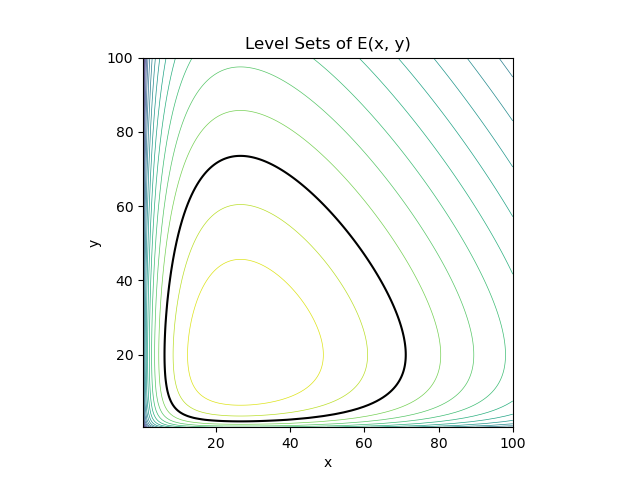
\includegraphics[width=250pt]{LV-levelsets.png}	
		\end{center}

		\item When plotting these with the same initial conditions, you should be clear that the Euler simulation doesn't give periodic solutions, as the errors make the simulation spiral out.
		
		Runge-Kutta however, gives periodic orbits.
		
		
	\end{enumerate}
		
	
\end{enumerate}
	
	
	
	
\item
\begin{enumerate}
	\item  We can see that to recover the original Lotka-volterra model, we need to ``remove'' the extra term, which will happen in the limit as $K \to +\infty$.
	
	\item The new system has three equilibrium solutions:
	\begin{itemize}
		\item $x=y=0$: Extinction
		\item $x=K, y=0$: Predator extinction with ideal prey population
		\item $x=1, y=\frac{K-1}{K}$, for $K\geq 1$: Co-existence
	\end{itemize}
	
	\item The Jacobian is
	\[
	J = \begin{bmatrix}
		-py+a\left(1-\frac{2x}{K}\right) & -px \\
		qy & qx-b
	\end{bmatrix}
	= \begin{bmatrix}
		-y+\left(1-\frac{2x}{K}\right) & -x \\
		y & x-1
	\end{bmatrix}
	\]
	
	So for each equilibrium we have:
	\begin{itemize}
		\item $x=y=0$: Eigenvalues $\pm 1$, so it is repelling unstable (saddle point)
		\item $x=K, y=0$: Eigenvalues $-1<0$ and $-(K-1)<0$, so it is attracting stable
		\item $x=1, y = \frac{K-1}{K}$: 
		\begin{itemize}
			\item[] $1 < K \leq  \frac12+\frac{1}{\sqrt{2}}$: Negative eigenvalues, so it is attracting and stable
			\item[] $K > \frac12+\frac{1}{\sqrt{2}}$: Real part of eigenvalues $<0$, so it is attracting stable (spiral sink)	
		\end{itemize}
	\end{itemize}

	\item 
	
\end{enumerate}	
\end{enumerate}
